\label{ch3:design_and_implementation}

\section{Design Targets}
The objective of this work is to design and implement a Network-on-Chip (NoC) router for a $3 \times 3$ mesh system. The target mesh structure is illustrated in Figure~\ref{fig:mesh_3x3_pe}. The router is designed to support packet-based communication using fixed-width flits and deterministic XY routing, while also providing virtual-channel-based flow control.

\begin{figure}[htbp]
    \centering
    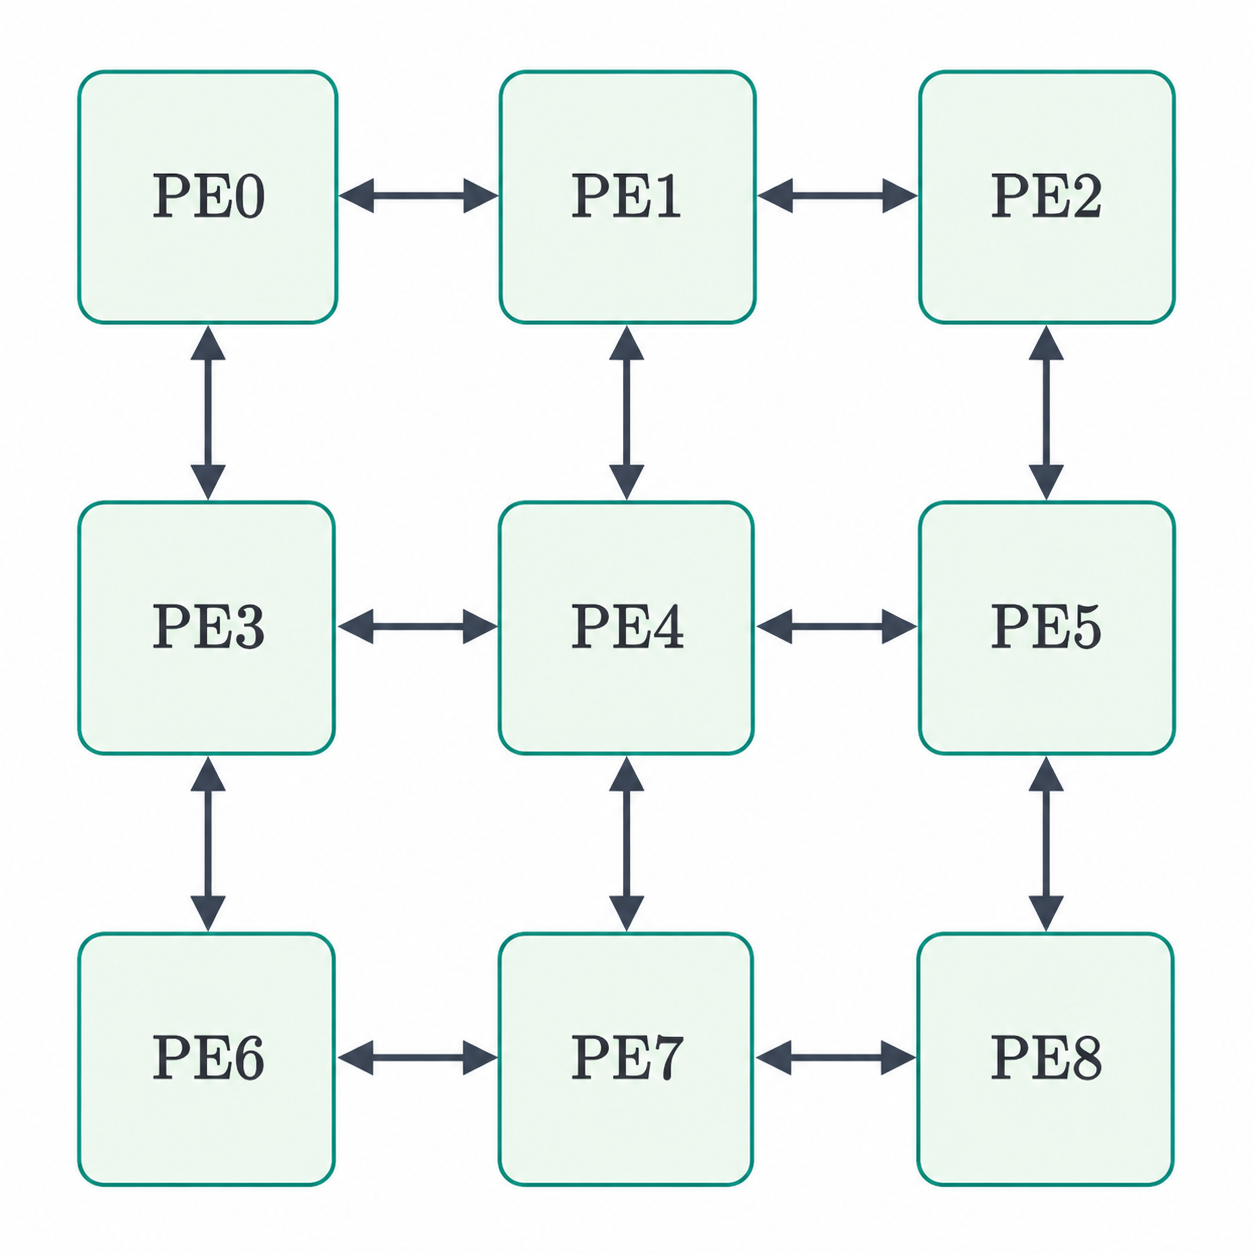
\includegraphics[width=0.4\textwidth]{images/ch3_design_and_implementation/3_times_3_mesh.png}
    \caption{$3 \times 3$ mesh structure}
    \label{fig:mesh_3x3_pe}
\end{figure}

The router first needs to provide the basic packet forwarding function. Each packet is sent from a source processing element to a destination processing element, and the routing decision is made according to the information carried in the header flit. Since a packet is divided into several flits, the router also has to make sure that flits belonging to the same packet follow the same reserved path and keep their original order. 

To organize the router operation, a three-stage pipeline is used. The first stage performs routing computation and virtual-channel allocation. The second stage is responsible for switch allocation, where the router decides which input can access the requested output port. The third stage performs switch traversal and sends the selected flit to the output side. By separating these functions into different stages, the design avoids putting too much logic into a single cycle and makes the implementation easier to meet timing.

Flow control is another important requirement in the router design. Since downstream buffers may become full, the router must be able to stop sending flits when the next router cannot accept more data. For this reason, the interface uses a valid-ready handshake together with credit-based flow control. A flit is transferred only when both valid and ready are asserted, while the returned credit information is used to indicate available buffer space in the downstream virtual channels.

Overall, the goal of this chapter is to present not only the implemented router structure, but also the design method used to connect routing decisions, virtual-channel allocation, flow control, and hardware implementation in a consistent router architecture.
\section{Router Architecture}
The design is based on a $3 \times 3$ two-dimensional mesh topology, in which nine processing elements are interconnected by routers. Each router contains five ports: one local port connected to the processing element, and four directional ports connected to the north, south, west, and east neighbors. This topology provides the communication framework for packet transmission in the target system.

Figure~\ref{fig:router_microarchitecture} illustrates the overall architecture of the proposed router. The router is designed to support flit-based packet forwarding under wormhole switching and virtual-channel flow control. In general, the router consists of routing computation, virtual-channel allocation, switch allocation, and switching logic, together with the required state management units. These modules cooperate to determine the output direction, assign channel resources, and transfer flits from the selected input side to the corresponding output side.The following sections describe the structure and implementation of these modules in more detail.

\begin{figure}[htbp]
    \centering
    \includegraphics[width=0.9\textwidth]{images/ch3_design_and_implementation/router_microarchitec.png}
    \caption{Router microarchitecture}
    \label{fig:router_microarchitecture}
\end{figure}

\section{Parameter Definition}
The main configuration parameters of the proposed router are summarized as follows:

\begin{itemize}
    \item \textbf{Topology and Node Definition:}

    The design is based on a $3 \times 3$ two-dimensional mesh topology, in which nine processing elements communicate through interconnected routers. Each router is identified by its Cartesian coordinates (x,y), where each coordinate ranges from 0 to 2. This coordinate-based representation provides a direct way to identify the position of each node in the network. 

    \item \textbf{Port Configuration:}

    Each router contains five ports, including one local port connected to the processing element and four directional ports connected to the north, south, west, and east neighboring routers. This five-port organization defines the communication interface of the router in the target mesh network. 
\[
\texttt{port\_t} \in \{\texttt{LOCAL}, \texttt{NORTH}, \texttt{SOUTH}, \texttt{WEST}, \texttt{EAST}\}.
\]
    \item \textbf{Packet and Flit Configuration:}

    For data transmission, packets are divided into 32-bit flits. The supported flit types include head flits, body flits, tail flits, and head-tail flits. Among them, the head flit carries the control and routing information required for packet forwarding. This information is organized into several header fields, including source and destination coordinates, flit type, packet length, virtual-channel information, and message-related fields. The header format and the detailed field definitions are shown in Figure~\ref{fig:header_format} and Table~\ref{tab:header_flit_fields}, respectively.
\[
\texttt{flit\_type\_t} \in \{\texttt{FLIT\_HEAD}, \texttt{FLIT\_BODY}, \texttt{FLIT\_TAIL}, \texttt{FLIT\_HEADTAIL}\}.
\]

\begin{figure}[htbp]
    \centering
    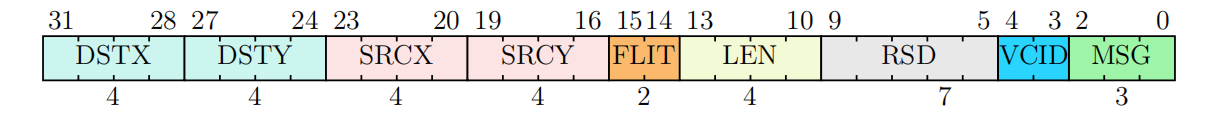
\includegraphics[width=0.8\textwidth]{images/ch3_design_and_implementation/header_flit_field.png}
    \caption{Header flit format and field definitions}
    \label{fig:header_format}
\end{figure}

\begin{table}[htbp]
    \centering
    \caption{Header Flit Fields}
    \label{tab:header_flit_fields}
    \begin{tabular}{llll}
        \hline
        \textbf{Field Name} & \textbf{Bit Slice} & \textbf{Width} & \textbf{Description} \\
        \hline
        DSTX & [31:28] & 4 & Destination ID. \\
        DSTY & [27:24] & 4 & Destination ID. \\
        SRCX & [23:20] & 4 & Source ID. \\
        SRCY & [19:16] & 4 & Source ID. \\
        FLIT & [15:14] & 2 & Flit Type. \\
        LEN  & [13:10] & 4 & Packet Length. \\
        VCID & [4:3]   & 2 & Next Hop IVC ID. \\
        MSG  & [2:0]   & 3 & Message Class. \\
        \hline
    \end{tabular}
\end{table}

    \item \textbf{Virtual Channel Configuration:}

    To support virtual-channel flow control, each router contains five ports, and each port is associated with both input-side and output-side virtual channels. Specifically, each input port contains four input virtual channels (IVCs), and each output port contains four output virtual channels (OVCs). Therefore, one router includes a total of 20 input virtual channels and 20 output virtual channels. These virtual channels provide the buffering and allocation resources required for flit storage, channel assignment, and packet forwarding in the router design.
\end{itemize}

\section{Handshake and Credit-based Flow Control}
The router adopts a two-way flow-control mechanism that combines a forward valid-ready handshake with backward credit return. The forward path transfers the flit data and its associated control information, while the backward path reports buffer-release events from the downstream router through \texttt{credit\_return}. Together, these mechanisms determine when a flit can safely move to the next router. This flow-control mechanism is illustrated in Fig.~\ref{fig:handshake_and_credit-based_flow_control}.

\begin{figure}[htbp]
    \centering
    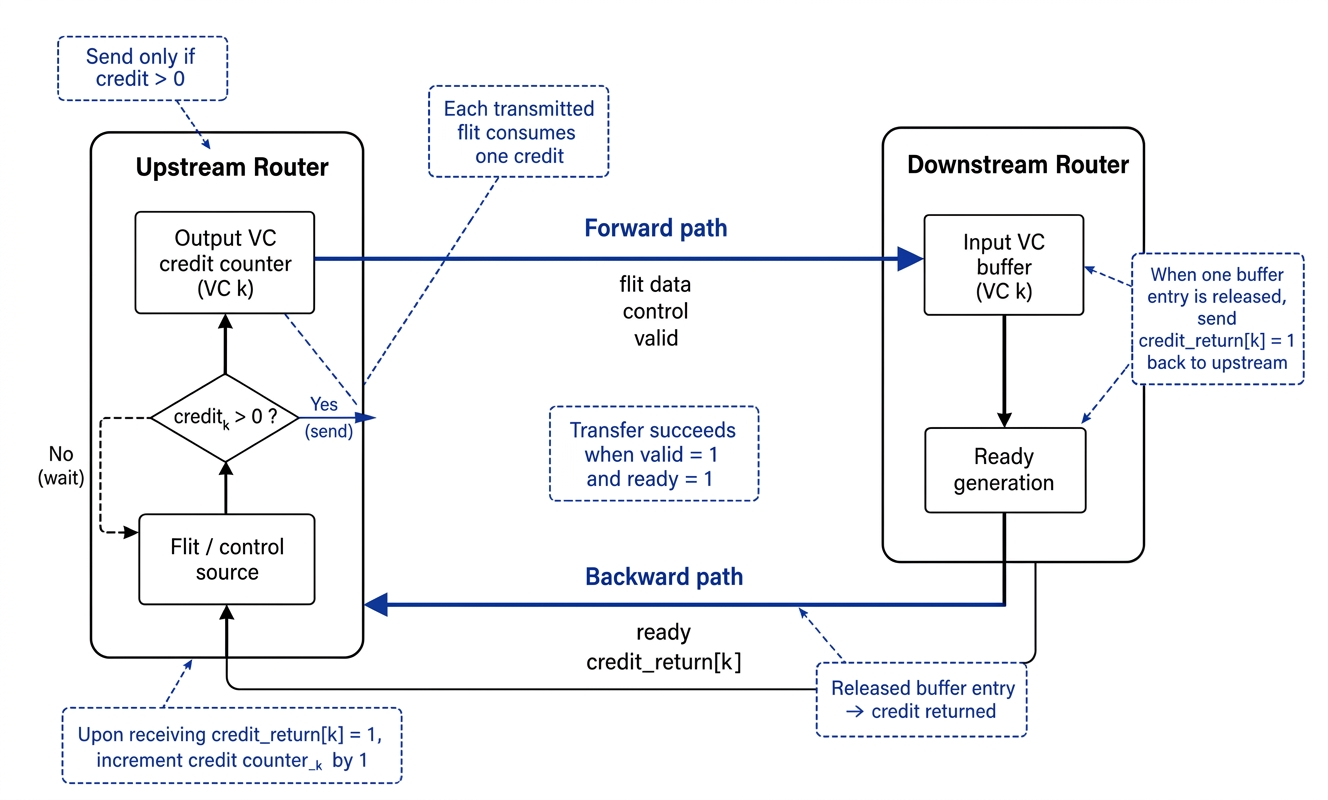
\includegraphics[width=0.85\textwidth]{images/ch3_design_and_implementation/handshake.png}
    \caption{Valid-ready handshake and credit-based flow control between neighboring routers.}
    \label{fig:handshake_and_credit-based_flow_control}
\end{figure}

In the forward path, a flit transfer is completed only when \texttt{valid} and \texttt{ready} are both asserted in the same clock cycle. The \texttt{valid} signal is generated by the sender to indicate that the current flit and its control fields are available, while \texttt{ready} is generated by the receiver to indicate that it can accept the flit in the current cycle. If \texttt{valid} is high but \texttt{ready} is low, the sender keeps the current flit and control signals stable until the handshake succeeds.

The credit return path is used to track the availability of downstream virtual-channel buffers. When \texttt{credit\_return[k] = 1}, one buffer entry in downstream input virtual channel \texttt{k} has been released. The upstream router then increments the corresponding output virtual-channel credit counter. Before scheduling a flit to an output virtual channel, the router checks whether the corresponding credit count is non-zero. A flit can be selected for transmission only when downstream buffer space is available, and each successful advancement consumes one credit.

In this design, the valid-ready handshake controls whether a flit is transferred in the current cycle, while the credit mechanism tracks downstream buffer availability across cycles. By combining these two mechanisms, the router avoids downstream buffer overflow and propagates backpressure when congestion occurs. This provides controlled and reliable flow-control behavior for pipelined flit transmission.

\section{Routing Algorithm}
The router uses a deterministic XY routing algorithm in the 3×3 mesh network. The output port is selected by comparing the current router coordinates with the destination coordinates in the header flit.

The packet is first routed in the X direction. If the destination is on the right, the packet is sent to EAST; if it is on the left, it is sent to WEST. When the X coordinate is already matched, the router then compares the Y coordinate and sends the packet to NORTH or SOUTH. If both coordinates match, the packet is delivered to the LOCAL port.

This method is simple and hardware-efficient, since it only requires coordinate comparison and no routing table. Another advantage is that XY routing naturally restricts all turns from the Y dimension back to the X dimension. Therefore, cyclic channel dependencies are avoided, which helps prevent routing deadlock. Its limitation is that the path is fixed and cannot adapt to congestion.

\begin{algorithm}[htbp]
\caption{Pseudo code of the XY-routing computation}
\label{alg:xy_routing}
\textbf{Definitions:}

\begin{itemize}
    \item $cur_x, cur_y$: current router coordinates.
    \item $dst_x, dst_y$: destination router coordinates.
    \item $port$: selected output port.
\end{itemize}

\textbf{Input:}

\begin{itemize}
    \item $cur_x, cur_y$: coordinates of current router.
    \item $dst_x, dst_y$: coordinates extracted from the header flit.
\end{itemize}

\textbf{Output:}

\begin{itemize}
    \item $port$: routing decision toward the next hop.
\end{itemize}

\begin{algorithmic}[1]
\If{$dst_x > cur_x$}
    \State $port \gets EAST$
\ElsIf{$dst_x < cur_x$}
    \State $port \gets WEST$
\ElsIf{$dst_y > cur_y$}
    \State $port \gets NORTH$
\ElsIf{$dst_y < cur_y$}
    \State $port \gets SOUTH$
\Else
    \State $port \gets LOCAL$
\EndIf
\State \Return $port$
\end{algorithmic}
\end{algorithm}


\section{Allocators and Arbiters}
In a NoC router, multiple flits may request the same limited resource in the same cycle. For example, several input virtual channels may request the same output virtual channel, or several input ports may try to access the same output port of the switch. Since each resource can only be used by one flit or packet at a time, arbitration is required to decide which request should be served.

An arbiter is used when multiple requesters compete for one shared resource. It receives several request signals and grants the resource to one selected requester. In contrast, an allocator handles a more general case where multiple requesters compete for multiple resources. Therefore, an allocator can be viewed as a structure built from several arbiters to generate a conflict-free matching between requesters and resources.

In this router, allocation is mainly used in two places. The first one is virtual-channel allocation, where input virtual channels compete for available output virtual channels. The second one is switch allocation, where flits from different input sides compete for access to output ports through the switch. Since these allocation steps are on the critical path of router operation, the allocator should be simple, fast, and suitable for hardware implementation. Therefore, this design uses a separable input-first allocation method based on round-robin arbiters.

\subsection{Round-robin Arbiter}
A round-robin arbiter is used as the basic arbitration unit in the allocator. The basic structure of the round-robin arbiter is shown in Figure~\ref{fig:rr_arbiter}. The round-robin arbiter used in this design is implemented using a rotating priority pointer and fixed-priority arbitration. The pointer \texttt{ptr} indicates the requester with the highest priority in the current arbitration round. Based on this pointer, the request vector is divided into a masked region and a wrap-around region. The masked request vector is first processed by a fixed-priority arbiter. If no active request exists in the masked region, the original unmasked request vector is arbitrated instead to complete the wrap-around selection.

\begin{figure}[htbp]
    \centering
    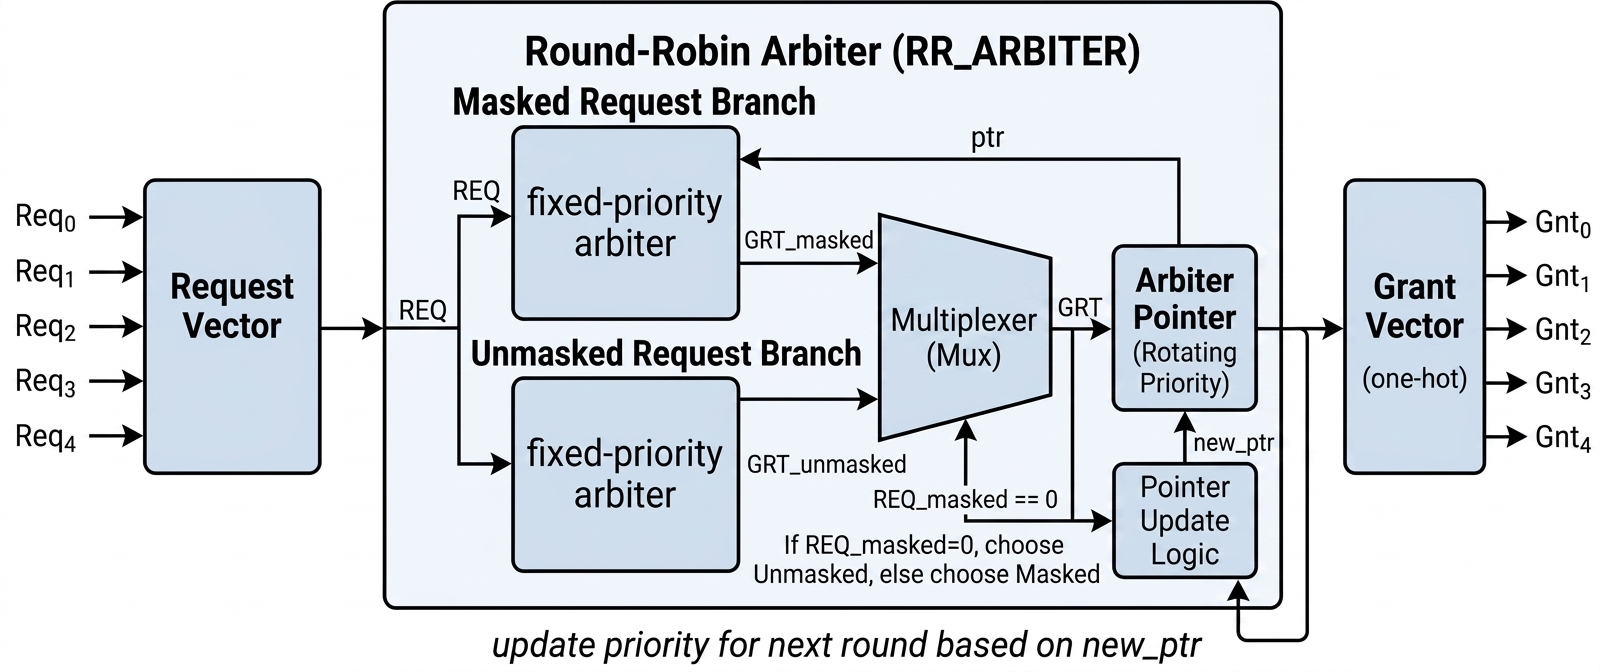
\includegraphics[width=0.85\textwidth]{images/ch3_design_and_implementation/round_robin_arbiter.png}
    \caption{Round-robin arbiter structure}
    \label{fig:rr_arbiter}
\end{figure}

After a grant is generated, the pointer is updated to the requester immediately following the granted one. Therefore, the winning requester is moved to the lowest priority position in the next arbitration round. When arbitration is not enabled or no request is active, the pointer remains unchanged. Compared with a fixed-priority arbiter, this rotating-priority mechanism provides better fairness, prevents one requester from continuously occupying the shared resource, and reduces the possibility of starvation.

\subsection{Separable Input-first Allocation}
A separable allocator is used to handle the case where multiple requesters compete for multiple resources. Instead of performing one large global arbitration, the allocation problem is divided into two simpler arbitration steps. This reduces hardware complexity and makes the allocator easier to pipeline and implement in RTL.

The allocator uses a separable input-first allocation strategy. The requesters are first grouped by input side. In the first arbitration step, each input side selects at most one candidate request from all its active requests. This means that one input can only forward one request to the second arbitration step in a given cycle. In the second step, each resource arbitrates among the candidate requests that target it and selects one final winner.

The overall organization of the separable input-first allocator is shown in Figure~\ref{fig:separable_input_first_allocation}. In this router, the separable input-first allocator operates on the requests from the virtual channels of five input ports. In the first level, each input-side arbiter selects at most one requesting virtual channel from the local VCs of the same input port. This produces one candidate request per input port. In the second level, the selected candidates are grouped according to their target output ports. Each output-side arbiter then selects one winning input among the candidates requesting the same output port. Since the router has five output ports, this stage ensures that each output port accepts at most one input in one cycle. Finally, the selected winners are mapped back to the original virtual channels to generate the final grant signals. In this way, the allocator guarantees that each input port grants at most one VC and each output port is assigned to at most one input.

\begin{figure}[htbp]
    \centering
    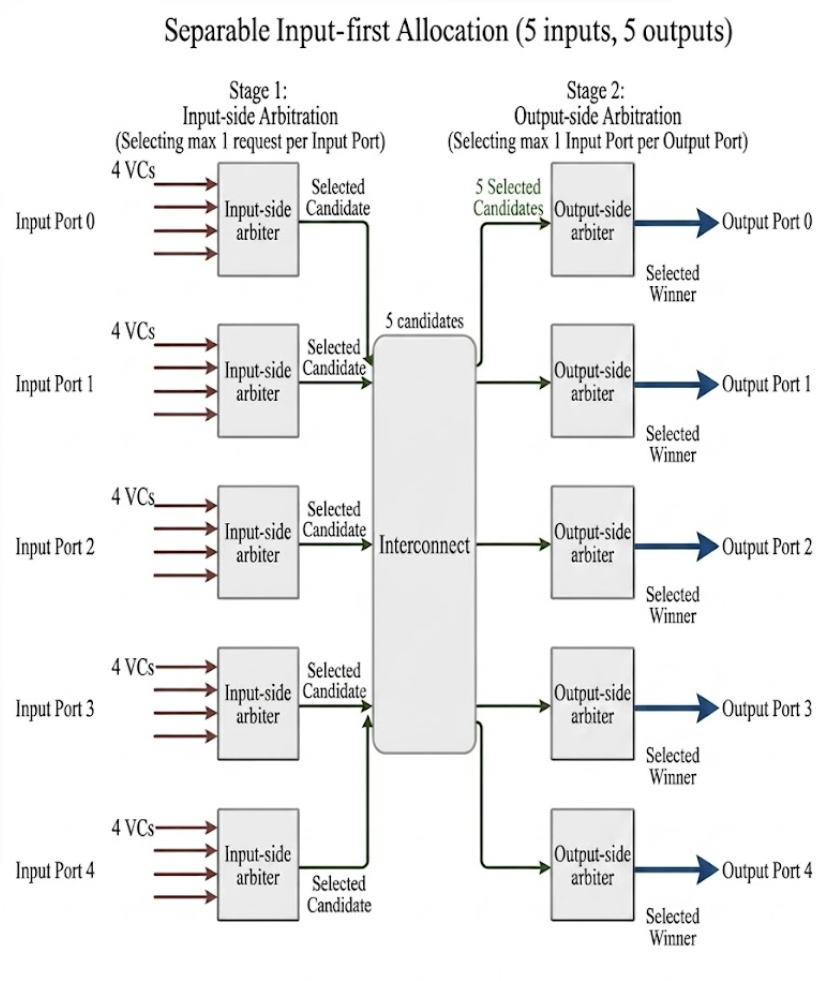
\includegraphics[width=0.8\textwidth]{images/ch3_design_and_implementation/Separable_Input_first_Allocation.png}
    \caption{Separable input-first allocation structure}
    \label{fig:separable_input_first_allocation}
\end{figure}

Figure~\ref{fig:separable_input_first_example} illustrates an example of separable input-first allocation with five inputs and five output resources. In Figure~\ref{fig:separable_input_first_example}(a), the request matrix shows all active requests before arbitration. After the first-stage input-side arbitration, each input keeps at most one selected request, forming the intermediate matrix shown in Figure~\ref{fig:separable_input_first_example}(b). The second-stage output-side arbitration then resolves conflicts among requests targeting the same output resource, and the final grant matrix is shown in Figure~\ref{fig:separable_input_first_example}(c). The final grant matrix contains only conflict-free grants, where each input receives at most one resource and each resource is assigned to at most one input.

\begin{figure}[htbp]
    \centering
    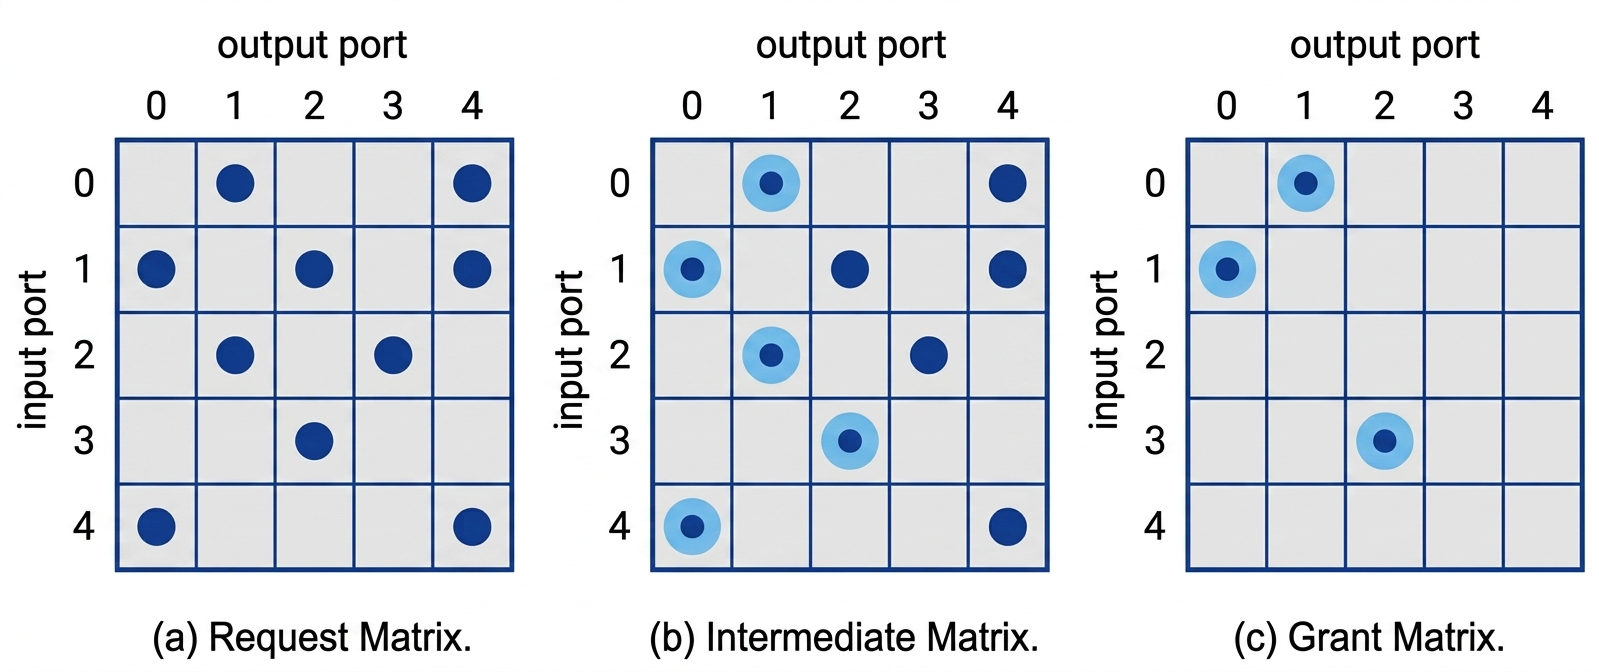
\includegraphics[width=0.9\textwidth]{images/ch3_design_and_implementation/matrix.png}
    \caption{Example of separable input-first allocation.}
    \label{fig:separable_input_first_example}
\end{figure}

The allocation result must still satisfy the basic matching rules: one requester can receive at most one grant, and one resource can be granted to at most one requester. Therefore, the final output of the allocator is a conflict-free grant result.

This approach is suitable for the router design because both virtual-channel allocation and switch allocation involve many requesters and multiple possible resources. By decomposing the allocation into two stages, the design avoids a large centralized allocator and keeps the arbitration logic relatively simple. The drawback is that separable input-first allocation may not always generate the maximum possible number of grants, because the first-stage arbiters make local decisions without knowing the final result of the second stage. However, this trade-off is acceptable for this design, since the main goal is to keep the router simple, predictable, and hardware-efficient.
\subsection{Virtual Channel Allocation}
The virtual-channel allocator is responsible for assigning an available output virtual channel to an input virtual channel. VC allocation is only performed for head flits. When the front flit of an input VC is a head flit, the allocator uses the routing result to identify the requested output port and checks the available output VCs at that port. The availability information is then combined with the candidate VC set to form the final set of allocatable output VCs.

If at least one valid candidate output VC exists, the corresponding input VC sends a request to the separable input-first allocator. The separable allocator then resolves competition among input VCs and output resources using the two-stage arbitration method described previously. When an input VC wins the allocation, the VC allocator generates a grant signal and a one-hot selected output VC signal for that input VC.

After a successful allocation, an update signal is sent to the state unit to mark the selected output VC as occupied. In this way, the VC allocation process can be summarized as three steps: candidate filtering, separable input-first arbitration, and output VC state update. Figure~\ref{fig:vc_allocation_flow} provides an overview of this allocation flow and the relationship among these three stages.

\begin{figure}[htbp]
    \centering
    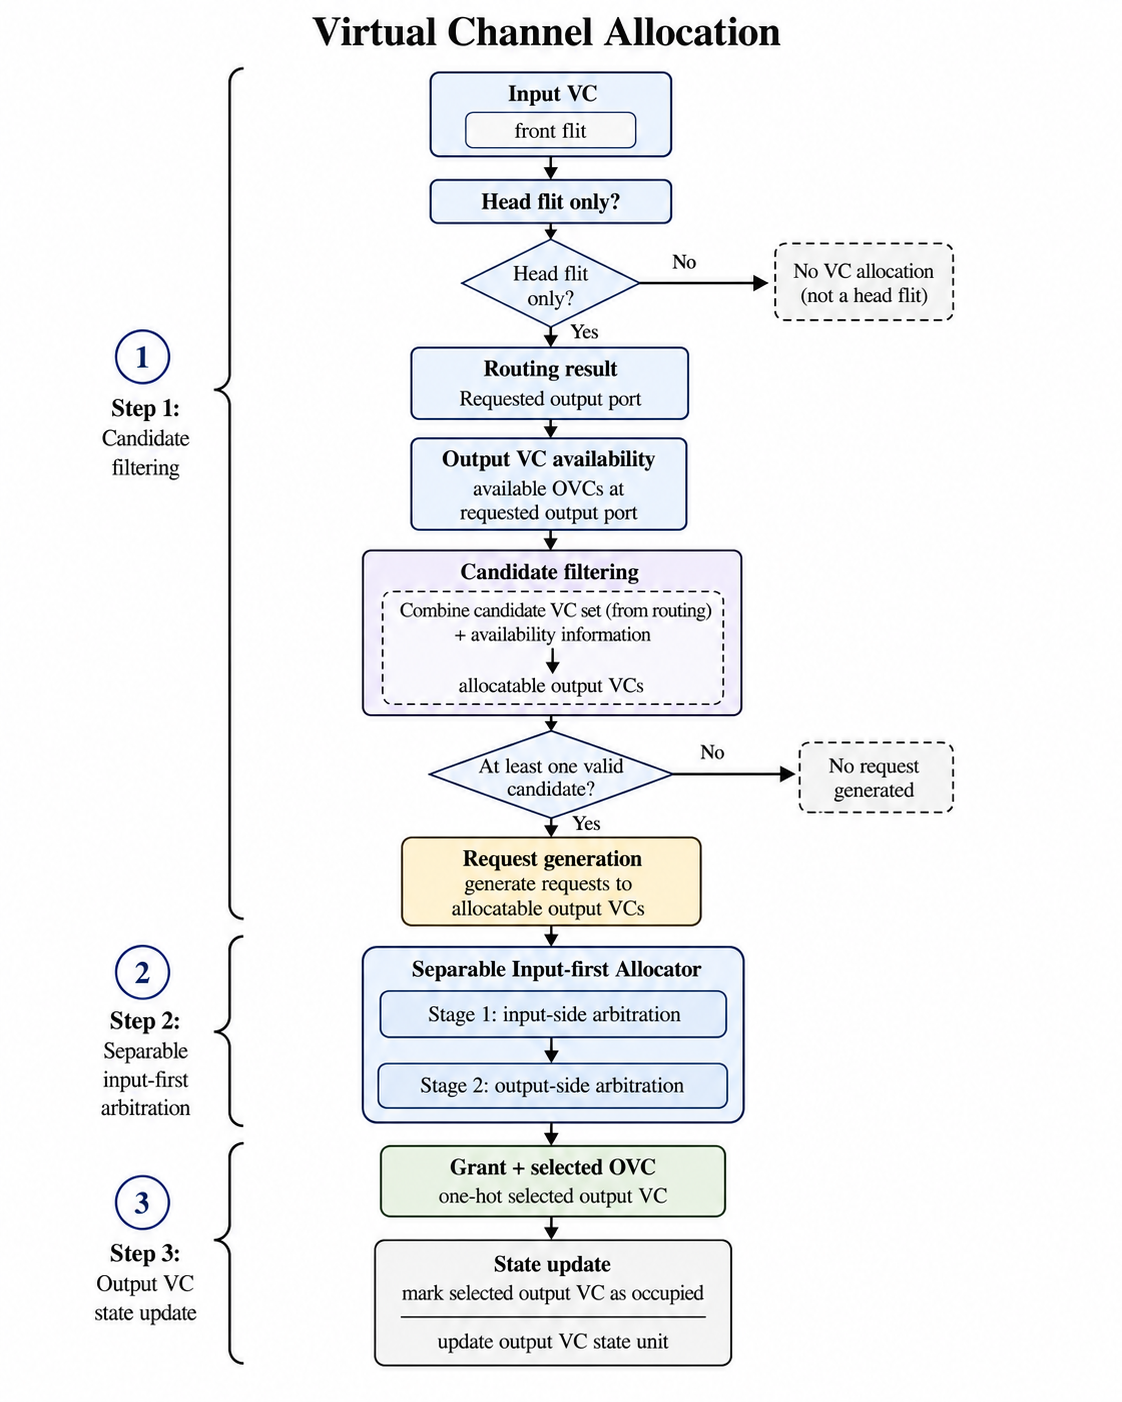
\includegraphics[width=0.8\textwidth]{images/ch3_design_and_implementation/virtual_channel_allocation.png}
    \caption{Virtual-channel allocation flow}
    \label{fig:vc_allocation_flow}
\end{figure}

\subsection{Switch Allocation}
After virtual-channel allocation assigns an output port and an output virtual channel to a packet, each flit of the packet still needs to obtain permission to traverse the router switch. This permission is determined by the switch allocator. In each cycle, the switch allocator selects the input flits that are allowed to access the crossbar and generates the corresponding switch control signals.

The switch allocation process follows the same separable input-first idea introduced earlier. Each input port first arbitrates among its local virtual channels and selects at most one flit that is ready to move forward. As a result, only one request from each input port can be sent to the output side in a cycle. The selected requests are then grouped according to their target output ports. If several input ports request the same output port, the output-side arbiter grants only one of them. The winning input-output pair is then used to configure the crossbar traversal path for that cycle. Figure~\ref{fig:switch_allocation_flow} summarizes the overall switch allocation procedure.

Credit availability is also considered before a flit is allowed to participate in switch allocation. A flit is considered ready only if its assigned downstream virtual channel has available buffer space. When a flit is successfully selected and moves forward, the corresponding credit is consumed. Therefore, switch allocation is not only responsible for crossbar scheduling, but also works together with credit-based flow control to avoid sending flits into a full downstream buffer.

Overall, switch allocation determines the cycle-by-cycle movement of flits through the router. It ensures that each input port sends at most one flit and each output port receives at most one flit in a cycle, while maintaining correct backpressure behavior through credit checking.

\begin{figure}[htbp]
    \centering
    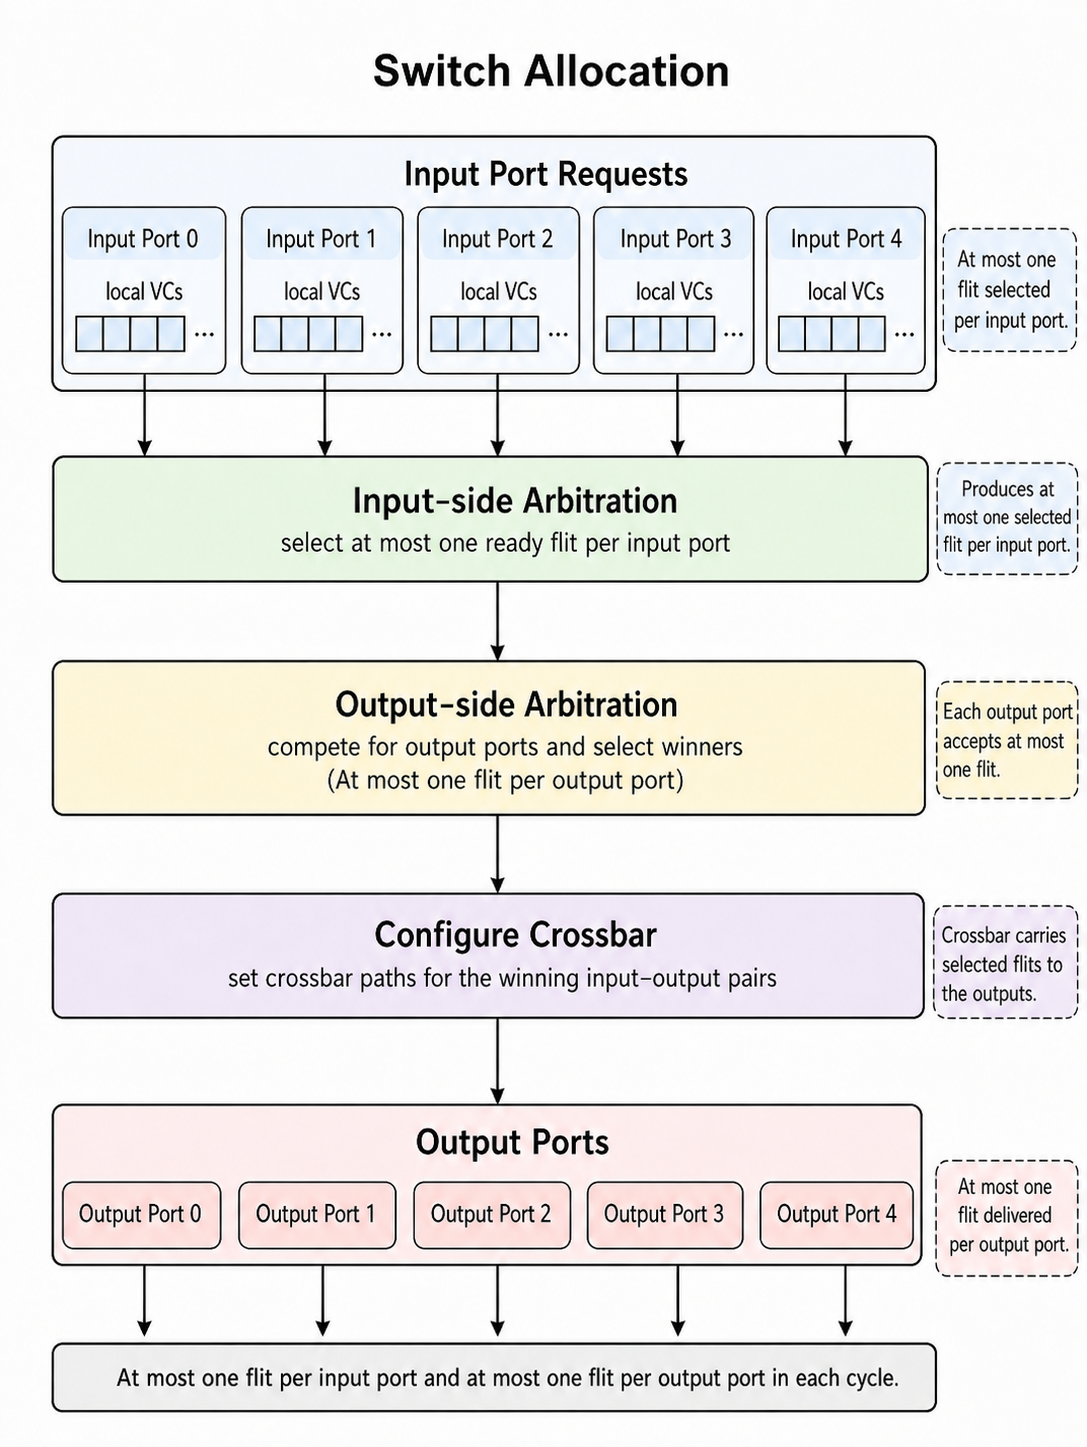
\includegraphics[width=0.6\textwidth]{images/ch3_design_and_implementation/switch_allocation.png}
    \caption{Switch allocation flow}
    \label{fig:switch_allocation_flow}
\end{figure}


\section{Pipeline Organization}

\subsection{Stage 1: Routing Computation and Virtual-channel Allocation}
In the first stage, the router inspects the front flit of each input virtual-channel FIFO. The front flit can be checked without being immediately removed from the buffer. If the front flit is a head flit and the corresponding input VC is not already locked by a previous packet, the router decodes the destination information from the header and performs XY routing to determine the requested output port.

After the output port is determined, the router tries to allocate an available output virtual channel at that port. If the allocation succeeds, the selected output port and output VC are stored in the first-stage pipeline registers. At the same time, an input-VC lock is established. This lock records the reserved output port and output VC, so that the body and tail flits of the same packet can follow the same path without repeating routing computation and virtual-channel allocation.

\subsection{Stage 2: Switch Allocation}
The second stage performs switch allocation. Only input VCs with valid first-stage information are allowed to request access to the switch. Since multiple input VCs may request the same output port in the same cycle, arbitration is required.

The switch allocator uses the separable input-first allocation method described earlier. For each input port, at most one local VC can win the input-side arbitration. For each output port, at most one requester can win the output-side arbitration. When a flit wins switch allocation, it is dequeued from the selected input VC FIFO and stored in the second-stage pipeline registers together with its control information, selected output port, and output VC.

When the flit moves from this stage to the next stage, one downstream credit is consumed. If the dequeued flit is a tail or head-tail flit, the corresponding input-VC lock is cleared at the end of this stage, allowing the next packet in the same input VC to perform routing computation and virtual-channel allocation later.
\subsection{Stage 3: Switch Traversal}
The third stage performs switch traversal and drives the output link. The flit stored in the second-stage pipeline registers is forwarded to the selected output port and appears on the corresponding output interface with the allocated VC identifier.

A flit leaves the router only when the valid-ready handshake succeeds on the selected output link. If the transmitted flit is a tail or head-tail flit, the corresponding output VC is released, making it available for another packet. Returned credits from the downstream router are also processed in this stage to update the output-VC credit counters.